%%%%%%%%%%%%%%%%%%%%%%%%%%%%%%%%%%%%%%%%%
% Journal Article
% LaTeX Template
% Version 1.3 (9/9/13)
%
% This template has been downloaded from:
% http://www.LaTeXTemplates.com
%
% Original author:
% Frits Wenneker (http://www.howtotex.com)
%
% License:
% CC BY-NC-SA 3.0 (http://creativecommons.org/licenses/by-nc-sa/3.0/)
%
%%%%%%%%%%%%%%%%%%%%%%%%%%%%%%%%%%%%%%%%%

%----------------------------------------------------------------------------------------
%	PACKAGES AND OTHER DOCUMENT CONFIGURATIONS
%----------------------------------------------------------------------------------------

\documentclass[twoside]{article}

\usepackage{lipsum} % Package to generate dummy text throughout this template
\usepackage[french]{babel}

\usepackage[utf8]{inputenc}

\usepackage[sc]{mathpazo} % Use the Palatino font
\usepackage[T1]{fontenc} % Use 8-bit encoding that has 256 glyphs
\linespread{1.05} % Line spacing - Palatino needs more space between lines
\usepackage{microtype} % Slightly tweak font spacing for aesthetics

\usepackage[hmarginratio=1:1,top=32mm,columnsep=20pt]{geometry} % Document margins
\usepackage{multicol} % Used for the two-column layout of the document
\usepackage[hang, small,labelfont=bf,up,textfont=it,up]{caption} % Custom captions under/above floats in tables or figures
\usepackage{booktabs} % Horizontal rules in tables
\usepackage{float} % Required for tables and figures in the multi-column environment - they need to be placed in specific locations with the [H] (e.g. \begin{table}[H])
\usepackage{hyperref} % For hyperlinks in the PDF

\usepackage{lettrine} % The lettrine is the first enlarged letter at the beginning of the text
\usepackage{paralist} % Used for the compactitem environment which makes bullet points with less space between them
\usepackage{todonotes}
\usepackage{tabularx}
\usepackage{graphicx}

\usepackage{abstract} % Allows abstract customization
\renewcommand{\abstractnamefont}{\normalfont\bfseries}
\renewcommand{\abstractname}{Résumé} % Set the "Abstract" text to bold
\renewcommand{\abstracttextfont}{\normalfont\small\itshape} % Set the abstract itself to small italic text

\usepackage{titlesec} % Allows customization of titles
\renewcommand\thesection{\Roman{section}} % Roman numerals for the sections
\renewcommand\thesubsection{\arabic{subsection}.\arabic{subsection}} % Roman numerals for subsections
\titleformat{\section}[block]{\bfseries\large\scshape\centering}{\thesection.}{1em}{} % Change the look of the section titles
\titleformat{\subsection}[block]{\bfseries\large}{\thesubsection.}{1em}{} % Change the look of the section titles

\usepackage{fancyhdr} % Headers and footers
\pagestyle{fancy} % All pages have headers and footers
\fancyhead{} % Blank out the default header
\fancyfoot{} % Blank out the default footer
\renewcommand{\headrulewidth}{0pt} %pour enlever la ligne du header
%\fancyhead[C]{titre, date, noms...	} % Custom header text
\fancyfoot[RO,LE]{\thepage} % Custom footer text


%agrandissement de la zone de texte
\addtolength{\oddsidemargin}{-1cm}
\addtolength{\evensidemargin}{-1cm}
\addtolength{\textwidth}{2cm}

%pour les maths
\usepackage{amsmath}
\usepackage{amsfonts}

%----------------------------------------------------------------------------------------
%	TITLE SECTION
%----------------------------------------------------------------------------------------

\title{\vspace{-15mm}\fontsize{24pt}{10pt}\selectfont\textbf{Étude de la méthode TOFD}} % Article title

\author{
\large
{Alice \textsc{Dinsenmeyer} \& Thomas \textsc{Lechat}}\\[2mm] % Your name %\thanks{}
%\normalsize University of California \\ % Your institution
%\normalsize \href{mailto:john@smith.com}{john@smith.com} % Your email address
\vspace{-5mm}
}
\date{}

%----------------------------------------------------------------------------------------

\begin{document}

\maketitle % Insert title

\thispagestyle{fancy} % All pages have headers and footers

%----------------------------------------------------------------------------------------
%	ABSTRACT
%----------------------------------------------------------------------------------------

\begin{abstract}

\noindent

Ce document présente le rapport du travail effectué dans le cadre des travaux pratiques du cours de contrôle non-destructif du master 2. L'étude d'une plaque possédant une soudure aillant des défauts connues est contrôlée à l'aide de la méthode TOFD. L'identification des différents signaux acquis est faites au moyen d'un calcul simple des temps de vols des différentes ondes misent en jeu. Les inhomogénéités sont alors visibles car de nouveaux échos apparaissent quand l'onde se diffracte sur les défauts. Dans un second temps, une méthode de mesure simultanée de l'épaisseur ainsi que de la vitesse des ondes est présentée puis testée. Celle-ci est facile à mettre en place mais nécessite de prendre plusieurs mesures pour augmenter la précision.

\end{abstract}

%----------------------------------------------------------------------------------------
%	ARTICLE CONTENTS
%----------------------------------------------------------------------------------------

\begin{multicols}{2} % Two-column layout throughout the main article text

\section{Introduction}
Cette étude s'inscrit dans le cadre du cours de Master 2 de contrôle non destructif. Cette discipline regroupe tout les procédés permettant la caractérisation d'une pièce ou d'un matériau sans en altérer les propriétés. En particulier, un grand nombre de méthodes basées sur la propagation des ondes élastiques ont été développées.

Notre travail porte sur la méthode TOFD: "Time Of Flight Diffraction", c'est a dire: "mesure du temps de vol de l'onde diffractée". Celle-ci consiste à analyser les temps de vol d'un paquet d'onde acoustique s'étant diffractés sur les bords d'un défaut. Cette méthode permet donc de caractériser la géométrie du défaut en plus de confirmer ou d'infirmer son existence. Cette méthode à tout d'abord été développée par Maurice Silk  \cite{artfonda1} dans les années 1970'. Elle est reconnue comme particulièrement pertinente pour le contrôle des soudures. C'est sur ce dernier cas que porte notre étude.

%------------------------------------------------

\section{Description du banc de mesure}
La méthode TOFD est ici utilisée sur une plaque d'acier comportant déjà des défauts connus. Un émetteur génère une onde de volume qui se diffracte sur le défaut puis, un capteur mesure cette diffusion. Un schéma du dispositif expérimentale se trouve figure~\ref{schema1}.
\bigskip

\begin{figure}[H]
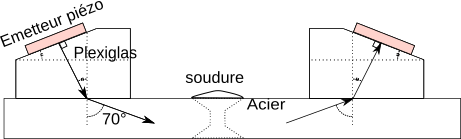
\includegraphics[scale=0.5]{./images/schema_expe.png}
\caption{\label{schema1} Schéma du banc d'expérience. }
\end{figure}

Les transducteurs utilisés sont des capteurs piézo-électriques Olympus (C544-SM) avec une bande passante centrée sur $10 MHz$ et d'une largeur de $6.35 mm$. Ces transducteurs sont montés sur des sabots Olympus (ST1-70L-IHC) permettant d'envoyer une onde longitudinale dans l'acier avec un angle d'incidente $\theta = 70 ^\circ$.

La plaque utilisée est de $20 mm$ d'épaisseur. En son centre se trouve une soudure dont les défauts sont connus à l'avance et répertoriés dans le tableau \ref{tab1}.
\bigskip

\begin{figure}[H]
\begin{tabular}{l|l|l}
Type de défaut & Taille & Position \\ \hline 
center line crack & 21 mm& 46 mm\\
lack of side wall fusion & 25 mm& 147 mm\\
Porosity & 27 mm& 213 mm
\end{tabular}
\caption{\label{tab1} Liste des défauts dans la soudure}
\end{figure}

Les mesures sont faites via un boîtier sonatest.

%------------------------------------------------

\section{Calcul des temps de vol des différentes ondes d’intérêts}
Afin de pouvoir déterminer quels ondes correspondent aux signaux des mesures, il est nécessaire de calculer les temps de vol de celles-ci. Trois types d'ondes interviennent dans la mesure: les ondes longitudinales (L) générées par la source, les ondes transversales (T) générées par conversion de modes lors de la réflexion sur l'arrière de la plaque, et enfin l'onde de tête (une onde L qui reste en surface). Les vitesses des différents types d'ondes sont dans un premier temps supposées connues ( $V_L = 5900 m/s$ et $V_T = 3200 m/s$). 

Afin de concentrer le maximum d'énergie au niveau des éventuels défauts, il est nécessaire de placer les transducteurs de tel sorte que les faisceaux se croisent au 2 tiers de l'épaisseur de la plaque. Les transducteurs doivent donc être placés à un distance $D = 2 \frac{2}{3}d tan(70^\circ)=72,5 mm $ l'un de l'autre. Les différents faisceaux sont représentés sur le schéma ~\ref{schema2}.

\bigskip
\begin{figure}[H]
\centering
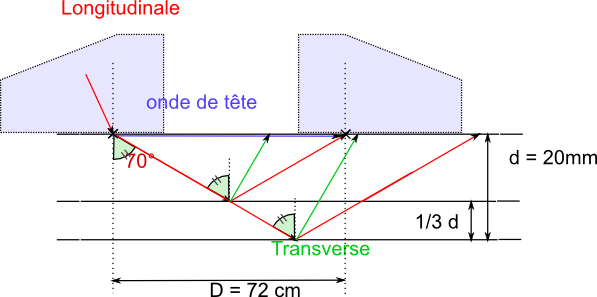
\includegraphics[scale=0.5]{./images/faiseaux.png}
\caption{\label{schema2} Schéma des parcours des différentes ondes pour une focalisation au 2 tiers du matériau et sans focalisation.}
\end{figure}

Après calculs, on obtient les distances et temps de vol répertoriés dans le tableau ~\ref{tab2} pour les différentes ondes mis en jeu dans le cas d'une réflexion sur un éventuel défaut et sans défaut.
\bigskip


\begin{figure}[H]
\begin{tabular}{l|l|l}
~ & distance & temps de vol \\ \hline
onde tête &$76 mm $& $ 12.8 \mu s$ \\
onde L &$ 116 mm $&$ 19,6 \mu s $\\
onde T &$ 78 mm $&$ 24,4 \mu s$ \\ \hline \hline
\end{tabular}

\begin{tabular}{l|l|l}
~ & distance & temps de vol \\ \hline
onde tête &$76 mm $& $ 12.8 \mu s$ \\
onde L &$ 78 mm $&$ 13.2 \mu s $\\
onde T &$ 54.2 mm $&$ 16.9 \mu s$
\end{tabular}

\caption{\label{tab2} Distance et temps de vol des faisceaux: Sans défaut puis avec défaut}
\end{figure}

Une première mesure est faite sur une partie de la plaque sans la soudure afin de pouvoir estimer l’imprécision de ces calculs. La figure \ref{fig1} représente les différents échos mesurés pour la configuration du dessus.

\begin{figure}[H]
\centering
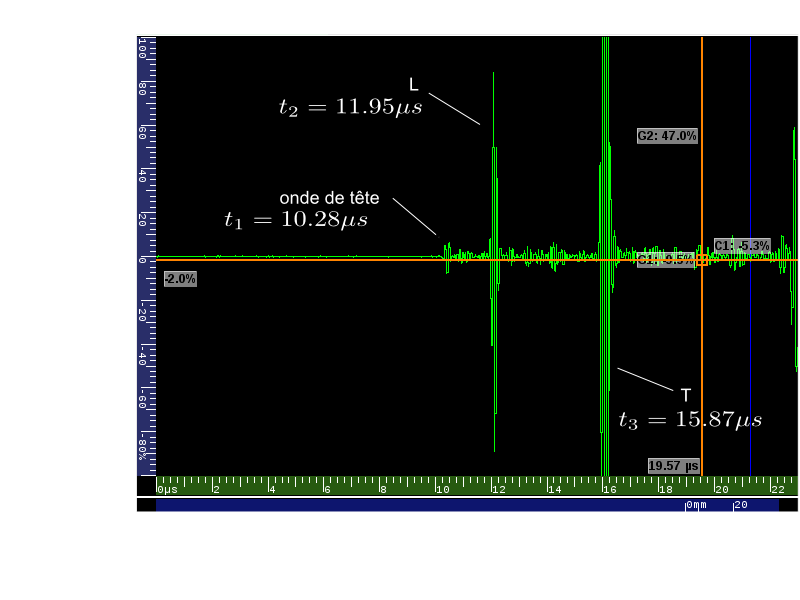
\includegraphics[scale=0.4]{./images/mesure_SD1.png}
\caption{\label{fig1} Mesure des temps de vol des différentes ondes pour une plaque de $20 mm$ d'épaisseur sans soudure ni défauts.}
\end{figure}

La mesure diffère de l'estimation faite précédemment: la largeur du faisceau n'a pas été prise en compte, or celle-ci n'est pas négligeable pour un capteur de $6mm$. La divergence du faisceau est elle aussi négligée. Enfin il manque au calcul précédent le temps nécessaire pour que les ondes L parcours les sabots à l'émission comme à la réception. Cependant, c'est surtout l'ordre des ondes qui importe: au vu des différents trajets (et des vitesses), l'onde de tête arrive en première puis vient la L et enfin la T. On peut donc facilement identifier ces ondes dans la suite.


%------------------------------------------------

\section{Scan de la soudure}
On utilise maintenant le dispositif sur la soudure. La figure ~\ref{fig2} montre les signaux pour un balayage sur toute la plaque. La mesure a été effectués 3 fois, les données aillant été quasi-identiques, seul la première mesure est présentée ici. Le gain est fixé à 60dB: les échos diffractés sont de bien plus faibles amplitudes que les signaux d'excitations, un gain élevé est donc nécessaire.

\begin{figure}
\centering
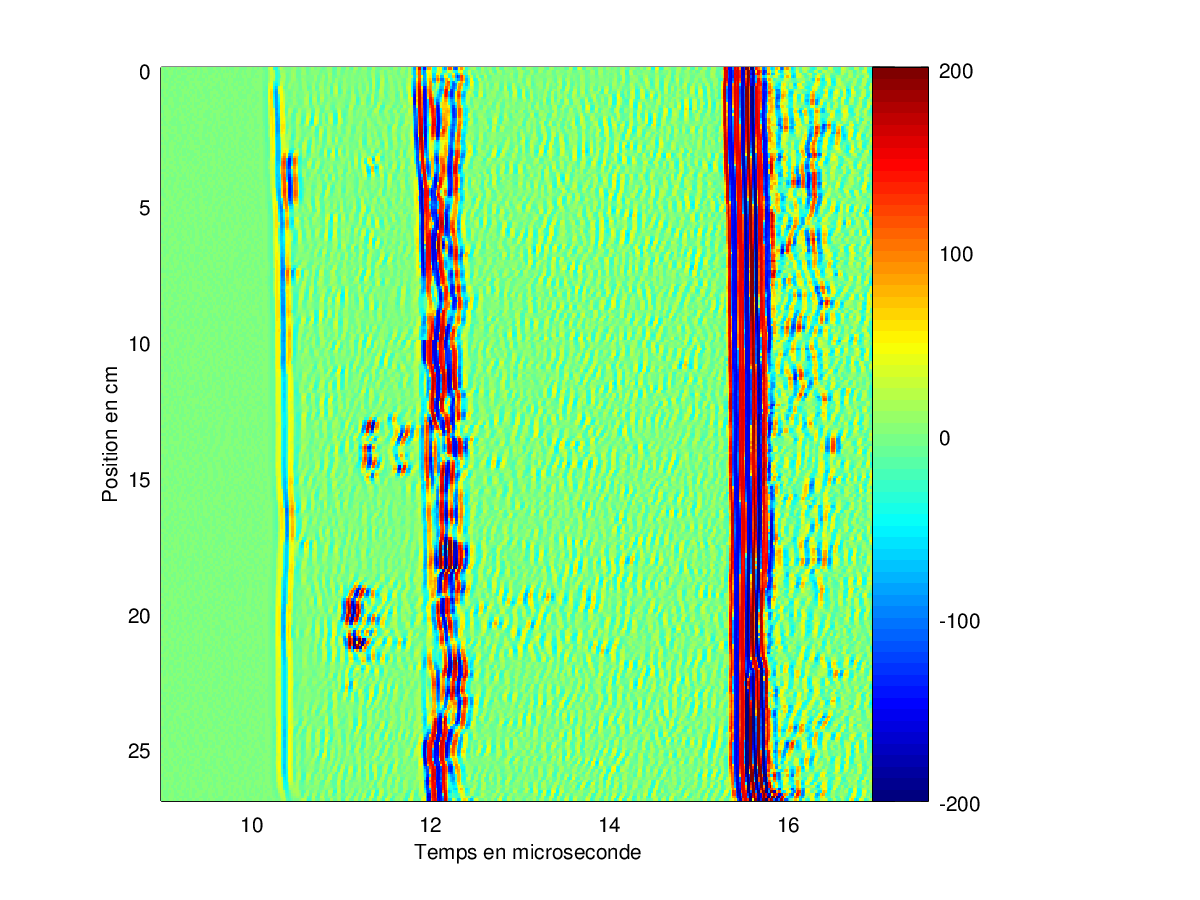
\includegraphics[scale=0.5]{./images/bscan.png}
\caption{\label{fig2} Scan d'une plaque avec une soudure possédant 3 défauts connus.}
\end{figure}

Des pics apparaissent bien aux endroits ou sont censés se trouver les défauts (tableau \ref{tab}). 
Le premier défaut se situe proche de la surface, l'onde de tête est donc plus affectée par celle-ci. La longueur du défaut est d'environ $20 mm$, se qui semble corroboré par la fiche technique des défauts dans la plaque.

Le troisième défaut est de type porosité, c'est pourquoi la tache est plus étendue que pour les 2 autres défauts: la multidiffusion des micro-bulles est bien visible. Là encore, la taille de la tache est bien celle présente dans la documentation.

 Enfin le deuxième défaut est visible sous la forme de 2 échos très rapprochés: ceux-ci correspondent en théorie à la diffraction par le bord supérieur ainsi que le bord inférieur du défaut, il est donc possible de remonter à la "largeur" du défaut (ou plutôt une projection de la largeur du défaut dépendant de l'angle entre l'incidence et le défaut). L'écart entre les 2 signaux est d'environ $dt = 0.4 \mu s$. On obtient donc un défaut d'une épaisseur de: $d = 0.4 *10^-6 V_L = 2.36 mm$ se qui ne semble pas invraisemblable. L'absence de cette information dans la documentation nous empêche de confirmer cette mesure.

\section{Mesure simultanée de la vitesse et de l'épaisseur par méthode de pitch\&catch}
Il n'est pas toujours facile de connaître l'épaisseur de la plaque ainsi que la vitesse de propagation des ondes ultrasonores dans celle-ci. Cette partie décrit une méthode
permettant de calculer ces 2 paramètres à l'issue de 2 mesures. Celle-ci est présentée dans l'article \cite{article1}: le but est d'effectuer 2 mesures de temps de vol dans un morceau de la plaque sain puis d'en déduire l'épaisseur ainsi que la vitesse des ondes à partir des formules suivantes:

\begin{eqnarray}
d = \frac{1}{2} \sqrt{ \frac{L_2^2 T_1^2 - L_1^2 T_2^2}{T_2^2	- T_1^2}} \\
v = \sqrt{\frac{L_2^2 - L_1^2}{T_2^2 - T_1^2}}
\end{eqnarray}

T1 et L1 correspondent au temps de vol ainsi qu'à la distance entre les transducteurs pour la configuration 1, T2 et L2 correspondent à la configuration 2. Le seul paramètre changeant d'une configuration à l'autre est la distance entre les capteurs (on doit avoir $L_2 > L_1$). La mesure faite précédemment pour une plaque sans soudure est reprise ici ($L_1 = 76mm$), une deuxième mesure est effectuée pour une distance $L_2 = 130 mm$. On obtient les paramètres suivants:
\begin{eqnarray}
T_1 = 12 \mu s , T_2 = 23.5 \mu s \\
L1 = 76mm , L2 = 130 mm \\
\leftarrow \left\{\begin{matrix}
d = 21.7 mm\\
 v= 5200m.s^{-1}
\end{matrix}\right. 
\end{eqnarray}

Le calcul de la distance est donc assez précise (moins de 10\% d'erreur) mais celui de la vitesse l'est moins. Une imprécision sur la mesure des temps de vol peut être à l'origine de ces imprécisions. Pour s'affranchir de se problème, les auteurs de l'article préconisent d'effectuer plus de mesures à différentes distances puis d'utiliser une méthode de moindre carré afin de grandement augmenter la précision de la mesure.

Contrôler l'épaisseur d'une plaque peut s'avérer utile par exemple dans le cadre du contrôle de cuves ou l'érosion est susceptible de ronger le conteneur.





\section{Conclusions et perspectives}
La méthode TOFD possède plusieurs avantages qui expliquent ça large utilisation dans les problématiques industriels: le scan peut être très rapide car 1 balayage suffit en principe pour contrôler toute une plaque (dans la pratique la zone se trouvant sous chaque capteurs n'est pas parcourue). De plus les dimensions du défaut peuvent être obtenus assez simplement: cela permet un suivis de l'endommagement de la pièce.

Cependant il ne faut pas perdre de vue que cette méthode à plusieurs inconvénients notables: les ondes diffractés sont de faibles amplitudes, c'est pourquoi il est difficile de détecter des petits défauts se trouvant sur la face opposée à celle parcouru par les transducteurs. Augmenter énormément le gain n'est pas une bonne solution car il apparaît alors un champ diffus liés au petites inhomogénéités du matériau. Or celles-ci ne sont pas des indicateurs de l'endommagement. Pour cette raison, cette méthode n'est pas adaptés au matériaux granulaires tel que le béton. De plus, dans la pratique, il peut être difficile d'évaluer les dimensions du défaut car si celui-ci est trop petit les différents échos sont confondus. Pour toutes ces raisons, la caractérisation des défauts nécessite une grande expérience de la part du technicien.

%----------------------------------------------------------------------------------------
%	REFERENCE LIST
%----------------------------------------------------------------------------------------

\begin{thebibliography}{99} % Bibliography - this is intentionally simple in this template
\bibitem[Silk1]{artfonda1}
M. G. Silk and B. H. Lidington, 1975 \\
\newblock \emph{ Defect  sizing  using  an Ultrasonic Time Delay Approach}
\newblock Br. J. NDT March ,pp.33–36


\bibitem[Silk2]{artfonda2}
M. G. Silk, 1979 \\
\newblock \emph{The transfer of ultrasonic energy in the diffraction technique for crack sizing}
\newblock Ultrasonics May, pp. 113–120


\bibitem[Silk3]{artfonda3}
M. G. Silk, 1997 \\
\newblock \emph{Sizing Crack-like Defects by Ultrasonic Means} 
\newblock In Research Techniques in Nondestructive Testing, Vol. 3, pp. 51–79, (1997), Academic Press, New York


\bibitem[YSSJ]{article1}
Young H Kim, Sung-Jin Song \& Jeong-Ki Lee, 2003 \\
\newblock \emph{ Simultaneous measurements of the ultrasonic wave velocity and thickness of a solid plate made from one side of the plate}




\end{thebibliography}

%----------------------------------------------------------------------------------------

\end{multicols}

\end{document}
